The proposed solution of the steady-state dynamic temperature estimation can be used in a wide range of optimization procedures. One of them is the reliability optimization that we discuss in this section. We perform a temperature-aware task mapping and scheduling in order to address the thermal cycling aging effect while keeping the energy consumption at an appropriate level. Both mapping and scheduling are based on a genetic algorithm \cite{schmitz2004}. Let us start with the overall description of the system.

\subsection{Application Model}
The system executes a periodic application with a set of data-dependent tasks. The overall structure of the application is defined by a task graph:
\begin{align*}
  & G = (\mathcal{V}, \: E, \: \mathcal{T}) \\
  & \mathcal{V} = \{ v_i: \: i = 0 \dots N_t - 1 \}
\end{align*}
where $\mathcal{V}$ is a set of $N_t$ vertices of the graph (tasks), $E$ is a set of edges (data dependencies between tasks), and $\mathcal{T}$ is the period of the application. Each pair of a task $v_i$ and processing element $\pi_j$ is characterized by a tuple $(C_{eff \; ij}, N_{cycles \; ij})$, where $C_{eff \; ij}$ is the effective switched capacitance and $N_{cycles \: ij}$ is the number of clock cycles. These parameters determine the processor load and execution time of the task, respectively.

\subsection{Temperature-Aware Reliability Model} \label{sec:reliability-model}
In the paper we address temperature-driven failure mechanisms with the reliability model presented in \cite{huang2009}, \cite{xiang2010}. The model is based on the assumption that the failure rate has a Weibull distribution (e.g., the thermal cycling, electromigration, etc. \cite{jedec2010}):
\[
  R(t) = e^{-(\frac{t}{\eta})^\beta}
\]
where $\eta$ and $\beta$ are the scaling and shape (slope) parameters, respectively. The mean time to failure (MTTF) for the Weibull distribution is given by the following equation:
\begin{equation} \label{eq:general-mttf}
  MTTF = \eta \; \Gamma(1 + \frac{1}{\beta})
\end{equation}
where $\Gamma$ is the gamma function. The shape parameter is found to be independent on the temperature variation \cite{chang2006}, which is not the case with the scaling parameter $\eta$. Therefore, the distribution can vary from one temperature to another. We can use the same approach as it was shown previously and split the overall period of the application $\mathcal{T}$ into $N_m$ time intervals $\Delta t_i$, so that during each time interval $\Delta t_i$ the corresponding $\eta_i$ is constant and equal to:
\begin{equation} \label{eq:eta-one}
  \eta_i = \frac{MTTF_i}{\Gamma(1 + \frac{1}{\beta})}
\end{equation}
where $MTTF_i$ is the mean time to failure of the $i$th time interval as if we had the failure distribution of this interval all the time. As it was shown in \cite{xiang2010}, the cumulative distribution function can be approximated as the following:
\[
  R(t) = e^{-(\frac{t}{\mathcal{T}} \sum_{i=0}^{N_m - 1} \frac{\Delta t_i}{\eta_i})^\beta}
\]
The formula keeps the form of the Weibull distribution with the scaling parameter equal to:
\begin{equation} \label{eq:eta-many}
  \eta = \frac{\mathcal{T}}{\sum_{i=0}^{N_m - 1} \frac{\Delta t_i}{\eta_i}}
\end{equation}
Consequently, $\eta$ can be substituted into \equref{eq:general-mttf} and the MTTF can be obtained. The only thing that is left is to determine $MTTF_i$ for each of the time intervals. In order to achieve this, we need to focus on the particular failure cause. As it was mentioned previously, the model can handle different failure mechanism; we have chosen the thermal cycling (TC) fatigue where the knowledge of the steady-state temperature in not sufficient and temperature curves should be investigated in details.

The number of thermal cycles to failure can be estimated using a modified version of the well-known Coffin-Manson equation with the Arrhenius term \cite{jedec2010}, \cite{xiang2010}, \cite{ciappa2003}:
\begin{equation} \label{eq:cycles-to-failure}
  \mathcal{N} = A (\Delta T - \Delta T_0)^{-b} e^{\frac{E_a}{k T_{max}}}
\end{equation}
where $A$ is an empirically determined constant, $\Delta T$ is the thermal cycle excursion, $\Delta T_0$ is the portion of the temperature range in the elastic region which does not cause damage, $b$ is the Coffin-Manson exponent with is also empirically determined, $E_{a}$ is the activation energy, $k$ is the Boltzmann constant, and $T_{max}$ is the maximal temperature during the thermal cycle. Having the number of cycles to failure and the duration of one cycle $\Delta t$, we can compute the MTTF that is missing in \equref{eq:eta-one}:
\begin{equation} \label{eq:mttf-cycle}
  MTTF = \mathcal{N} \; \Delta t
\end{equation}
Hence, taking equations \eqref{eq:general-mttf}, \eqref{eq:eta-one}, \eqref{eq:eta-many}, and \eqref{eq:mttf-cycle} together, we obtain the following expression to estimate the MTTF for the whole period of the application:
\begin{align} \label{eq:one-mttf}
  MTTF = \frac{\mathcal{T}}{\sum_{i=0}^{N_m - 1} \frac{1}{\mathcal{N}_i}}
\end{align}

\equref{eq:one-mttf} describes the MTTF of one component, which is a processing element in our case. We assume that each processing element is essential for the proper work of the system, therefore, a failure of any core leads to the total failure of the whole system. Consequently, the MTTF of the system can be estimated as the minimal MTTF among its components:
\begin{align}
  & MTTF_{sys} = \min_{i=0}^{N_p - 1} \; MTTF_i \label{eq:mttf-system} \\
  & MTTF_i = \frac{\mathcal{T}}{\sum_{j=0}^{N_{m \: i} - 1} \frac{1}{\mathcal{N}_{ij}}} \nonumber
\end{align}
where $N_{m \: i}$ is the number of thermal cycles of the $i$th processing element within the application period $\mathcal{T}$ and $\mathcal{N}_{ij}$ is the number of thermal cycles to failure as if the $j$th cycle was being repeated all the time.

\subsection{Motivational Example} \label{sec:motivation}
Consider an application with six tasks, denoted ``T0''--``T5'', and a heterogeneous architecture with two cores, labeled ``PE0'' and ``PE1''. The task graph of the application is given in \figref{fig:task-graph} along with the execution times for both cores. The period of the application is 0.06 seconds. A first alternative mapping and schedule, and the resulting SSDTP are shown at the top of \figref{fig:motivation} (where the hight of a task represents its relative dynamic power consumption). It can be observed that initially PE0 is experiencing three thermal cycles. If we change the mapping of T5 and move it to PE1, we achieve two thermal cycles of PE0 instead of three. Finally, if we vary the schedule as well and change the order of T1 and T3, the number of cycles of PE0 becomes one. Using the reliability model from \secref{sec:reliability-model}, we observe improvements in the MTTF of 44.69\% and 54.53\%, respectively, relative to the initial configuration.
\begin{figure}
  \centering
  \subfloat[The task graph.]{
    \label{fig:task-graph}
    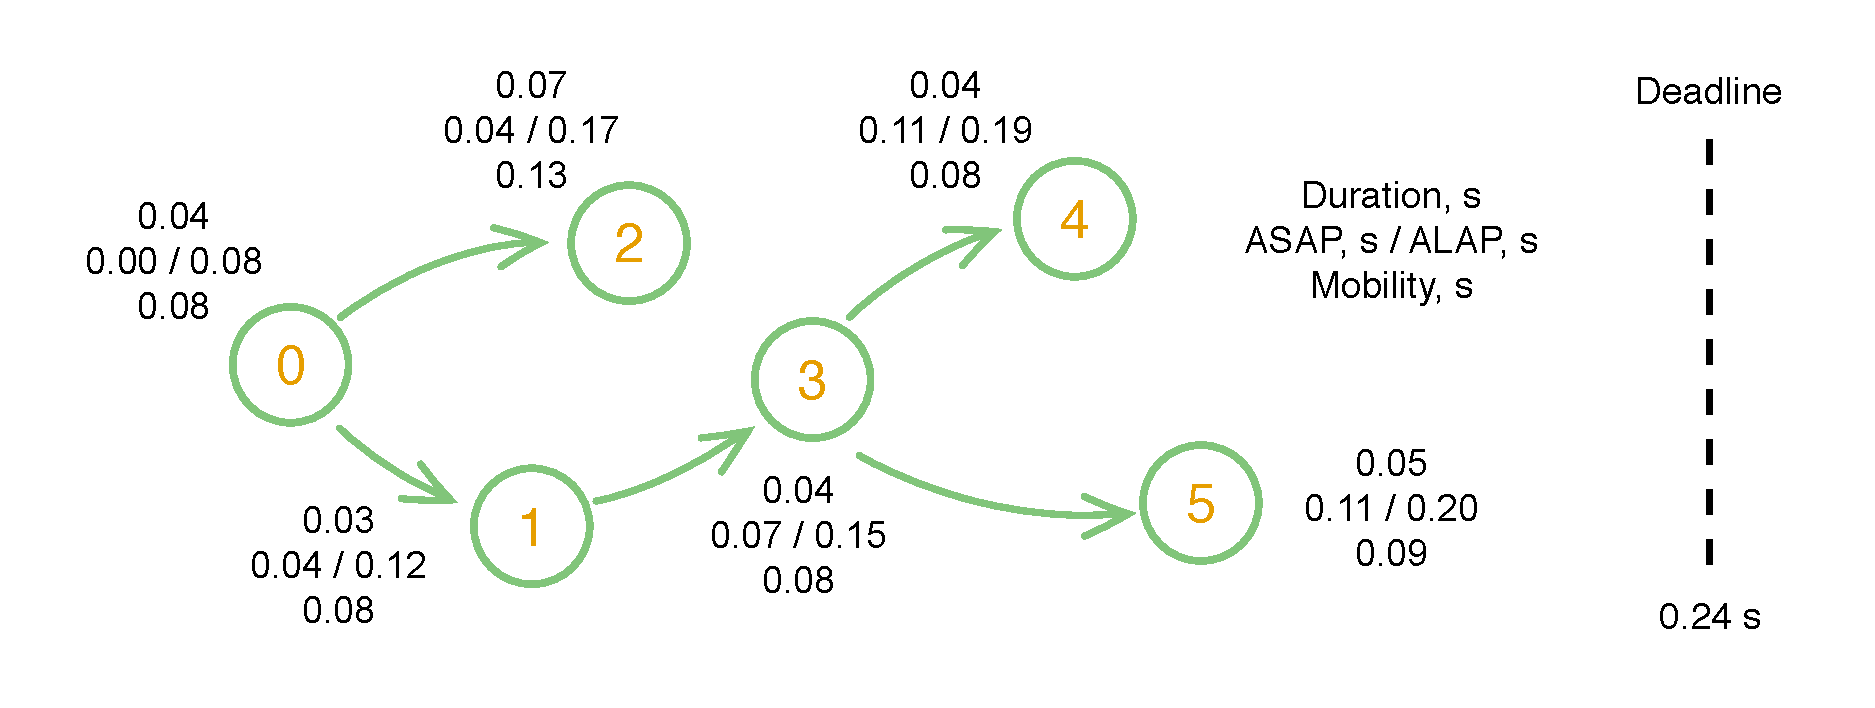
\includegraphics[width=0.8\linewidth]{assets/task-graph.pdf}
  }
  \vspace{-15pt}

  \subfloat[Alternative mappings and schedules.]{
    \label{fig:motivation}
    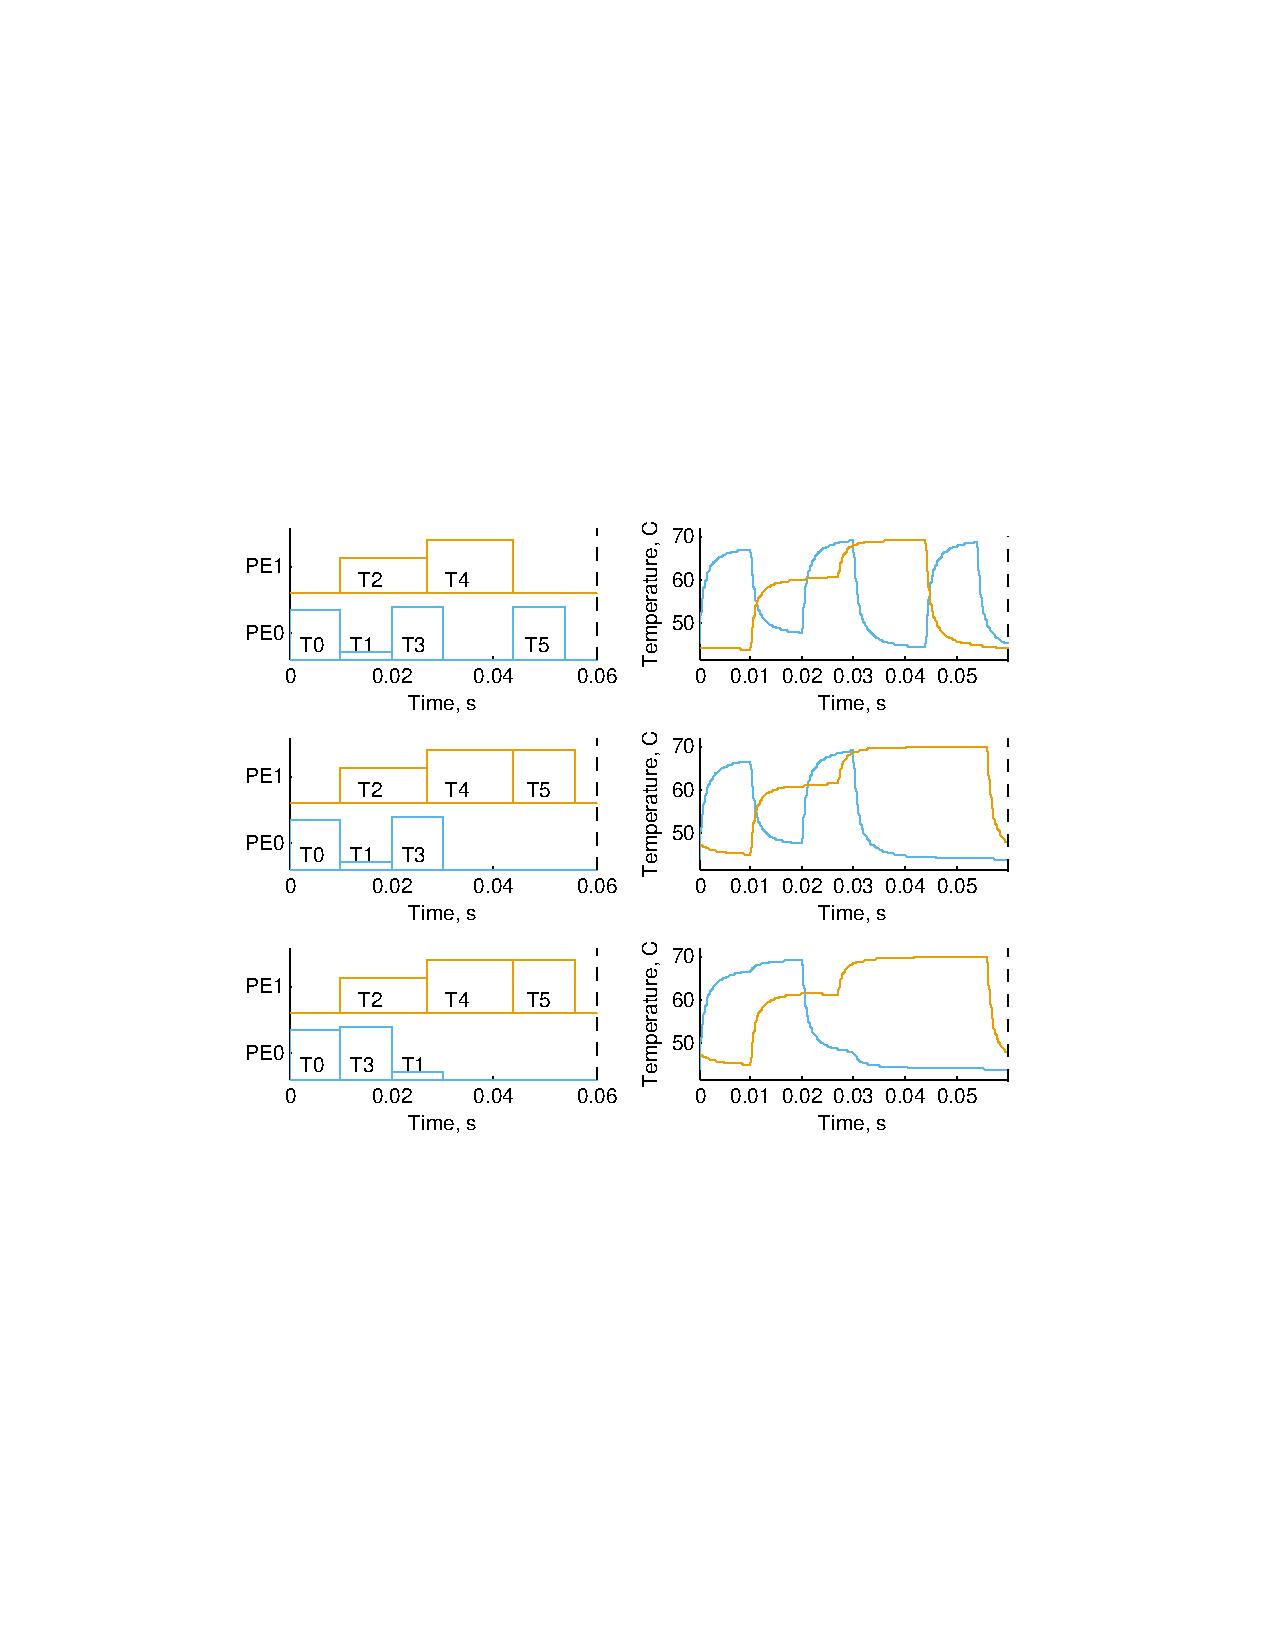
\includegraphics[width=0.8\linewidth]{assets/motivation.pdf}
  }
  \vspace{5pt}
  \caption{Motivational example.}
  \vspace{15pt}
\end{figure}


\subsection{Genetic Algorithm}
The optimization procedure is held by a genetic algorithm (GA) \cite{schmitz2004} that varies mapping and scheduling of the application in order to maximize the MTTF of the system. Each chromosome is a vector of $2 \times N_t$ elements, where the first half encodes priorities of the tasks and the second represents a mapping. The population contains $4 \times N_t$ individuals that are initialized partially randomly and partially based on the mobility of the tasks \cite{schmitz2004}. Each generation, a number of individuals, called parents, are chosen for breeding by the tournament selection with the number of competitors proportional to the population size. The parents undergo the 2-point crossover with $0.8$ probability and uniform mutation with $0.05$ probability. The evolution mechanism follows the elitism model where the best individual always survives. The stopping condition is an absence of improvement within $200$ successive generations.

A chromosome is evaluated in a number of steps. First, the decoded priorities and mapping are given to a list scheduler that produces schedules for each of the cores. If the schedules do not respect the deadline of the application, the solution is penalized proportionally to the delay and is not further evaluated; otherwise, based on the parameters of the architecture and tasks, a dynamic power profile is obtained. Having the dynamic power profile and taking into consideration the leakage power with the linear approximation from \secref{sec:leakage}, the corresponding SSDTP is computed by the CE method. Finally, the SSDTP is assessed in terms of the reliability model given in \equref{eq:mttf-system}, where the rainflow counting method is employed to count thermal cycles \cite{xiang2010}.
